\section{Server Design}

The GIM server is primarily responsible for synchronising the communication between the connected clients and keeping a persistent record of user information. In particular the server is responsible for:

\begin{itemize}
    \item{Authenticating users}
    \item{Routing chat messages for one client to one or more other clients}
    \item{Sending requests from one client to another client (such as friend requests or chat invites)}
    \item{Notifying subscribed users of changes to another user's information}
    \item{Storing user information such as nicknames, passwords, display pictures, friend lists, etc.}
\end{itemize}

\subsection{Key Concepts}

\subsubsection{User}
A user is a registered account on the server with a unique identifier (an email address), password, nickname, personal message, display picture, status, and friend list. 

\subsubsection{Identification}
The user's identifier and password are used to authenticate the user at login. These cannot be changed one the account has been created. 

\subsubsection{Nickname}
A user's nickname is a short and familiar name for that user. A nickname does not need to be unique and is not intended to be used as an identifier by the system. By default a user's nickname is their email address.

\subsubsection{Personal Message}
The personal message is a medium length message (usually only a sentence or two) which the user can use to share news or any information about themselves.

\subsubsection{Display Picture}
A Display Picture is a small image chosen by the user, often of themselves, so that they can be easily identified visually. By default a user's display picture is the GIM logo. 

\subsubsection{Status}
A user can have one of several statuses: Online, Away, Busy and Appear Offline. The first three statuses are used simply as an indication of the user's likelihood to respond to a message. The Appear Offline status allows the user to appear to other users as though they were not signed in but still receive updates and messages from other users.

\subsubsection{Friend List}
Each user has their own Friend List, a list of users who have accepted a friend request from the owner of the Friend List. When a user accepts a friend request, the sender and receiver are added to each other's Friend List. The server only grants access to information about a user if that user is in the requesting user's Friend List or if the users are currently in the same Room. This means that simply removing a user from your Friend List does not stop them from being able to view your information or message you.

A user is considered to be `subscribed' to all of the users in their Friend List. This means that they receive update notifications from the server whenever a user in their Friend List updates their nickname, personal message, display picture or status.

\subsubsection{Blocked User}
A user is able to stop a another user from communicating with them and viewing their information by blocking that user. It is possible to block any user, even users not currently in your friend list. Blocking a user is a one-way process and does not stop a user from messaging or viewing information about users they have blocked.

\subsubsection{Room}
A Room is a collection of one or more users and each Room has a unique identifier. All chat messages in GIM are sent to Rooms rather than particular users. The server then forwards messages from the room to the users in the room.

In order to join a Room a user must either create a new Room (in which case they are automatically placed into the Room) or they must be invited to the Room by a user already in the Room. 

A Room can be one of two types: Personal or Group. A Personal Room is much more restrictive than a Group Room. A Personal Room must be provided with the identifier of one other user at time of creation and is limited to only 2 users. Once a Personal Room has been created you cannot invite any other users. A Group Room has no such restrictions. Any number of users may be invited to a Group Room at any time.

\subsection{Server Structure}

From the very beginning the server was designed to be secure, scalable, and simple. Users must trust it to keep their information safe and route messages correctly, and it must be able to cope with any number of connected clients.

In order to manage this, the server generates a new worker for every connected client. This new worker acts as the single point of contact for its respective client. This greatly simplifies the design of the server as we can treat each connection individually and allows the server to easily scale to a large number of clients.

\begin{figure}[!h]
    \begin{center}
        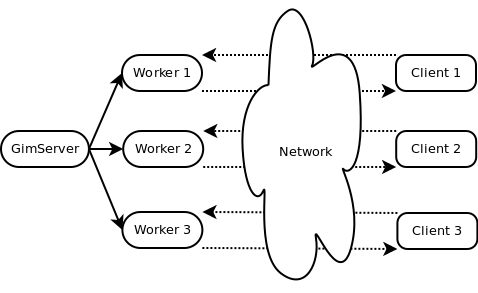
\includegraphics[scale=0.75]{chapter2/diagrams/server_workers.png}
        \caption{The GIM Server with 3 connected clients, each with their own worker.}
        \label{WorkersDia}
    \end{center}
\end{figure}

Each worker has 2 buffers, one which stores commands read from the network (the command buffer), and one which stores commands to be written to the network (the response buffer). The worker continually reads commands from the command buffer, processes them, and puts the responses into the response buffer. At the same time the worker is also reading and writing data from the respective buffers onto the network.

\begin{figure}[!h]
    \begin{center}
        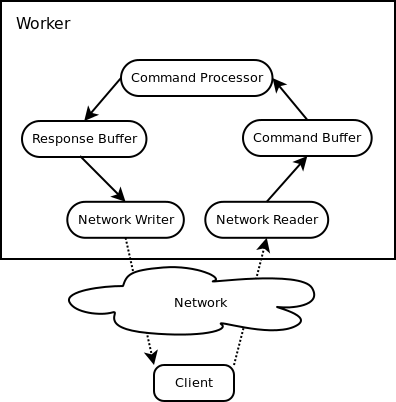
\includegraphics[scale=0.75]{chapter2/diagrams/worker_detail.png}
        \caption{A more detailed diagram of what happens inside a worker.}
        \label{WorkersDia}
    \end{center}
\end{figure}

Workers are able to indirectly communicate with other clients by putting commands into other workers' buffers. Since the command still passes through the worker assigned to the client, this allows a worker to pass requests and messages from one client to another without directly communicating with the other client.

Workers can also communicate using the shared data.


\begin{figure}[!h]
    \begin{center}
        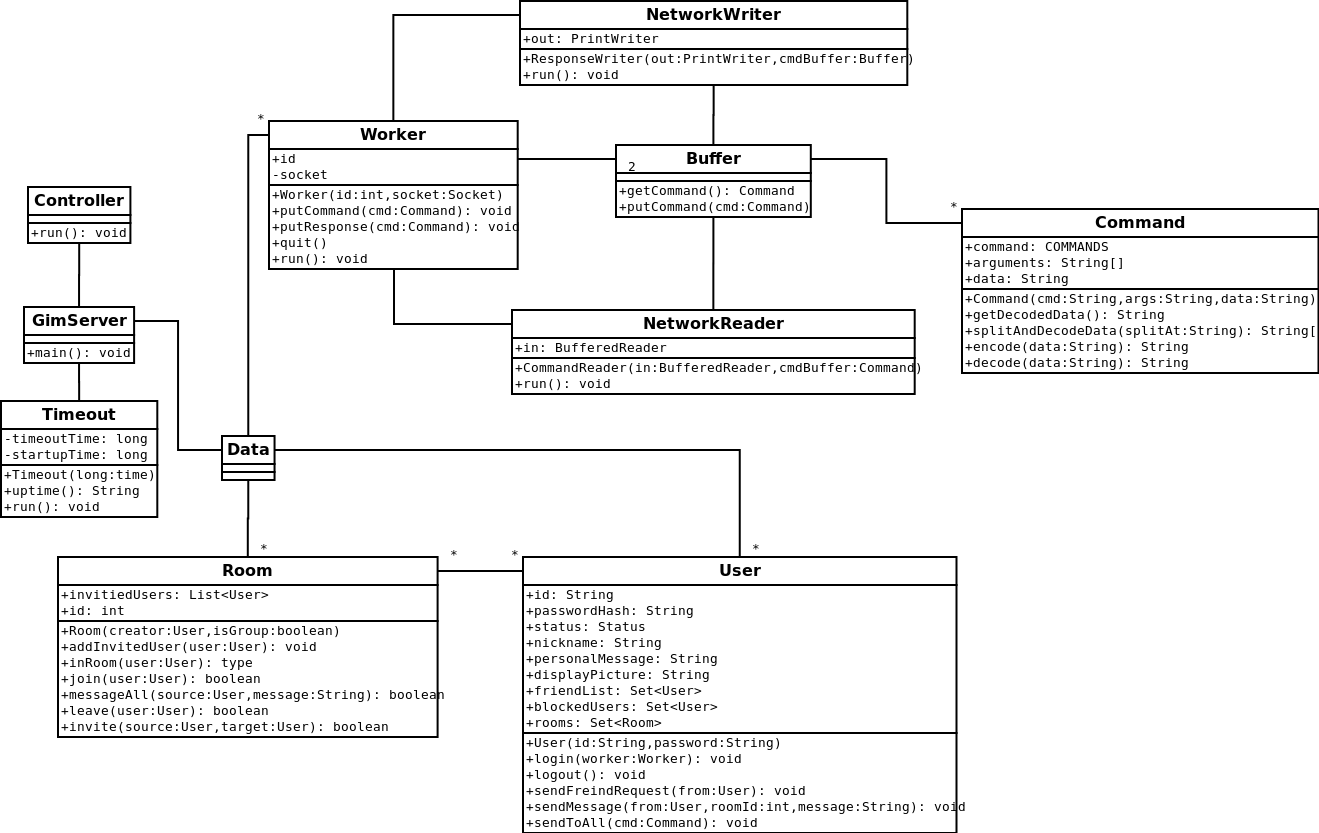
\includegraphics[scale=0.65]{chapter2/diagrams/server_uml.png}
        \caption{THIS IS NOT DONE.}
        \label{highLevelDia}
    \end{center}
\end{figure}

